\chapter{\acl{sota} Research}
\label{chapter:soa}

\section{Emotion}

The first step to building a successful \ac{ser} model is to have the concept of emotion carefully defined. There are various approaches to modeling emotions, and there is still no consensus on an accurate representation due to its natural subjectivity.

Currently, the main accepted and utilized for the emotion recognition task are the discrete and dimensional models.

\subsection{Discrete Emotion}

Discrete/categorical theories of emotions claim that some core emotions are characterized by stable patterns of triggers, behavioral expression, and associated distinct subjective experiences \cite{Hudlicka2017}.

The emotions considered in these theories are typically the \textit{basic} emotions, including happiness, sadness, fear, anger, disgust, and surprise.

Most of the existing systems focus on these basic emotional categories. Instinctively, people use this model in their daily life, consequently, models based on discrete labels are more intuitive.

\subsection{Dimensional Emotion}

The dimensional emotional model uses dimensions such as valence, arousal, control, or power, to characterize emotions. It represents emotions as coordinates in a multidimensional space. These dimensions are definitive and generic aspects of emotion. One of the most preferred dimensional models is a two-dimensional model, as shown in figure \ref{fig:emoValAro} below, that uses arousal or activation, versus valence or evaluation on the other \cite{Shuman2015}.


\begin{figure}
	\centering
	\begin{subfigure}{.5\textwidth}
		\centering
		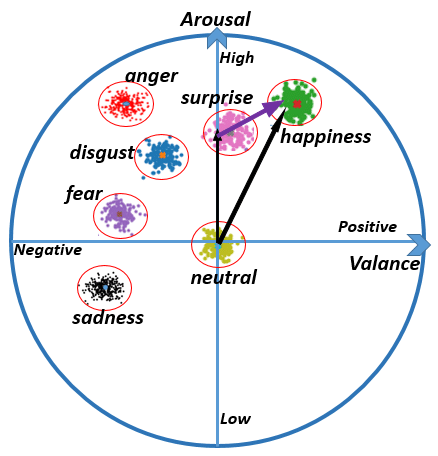
\includegraphics[width=.75\linewidth]{figs/2_state_of_the_art/emoValAro.png}
		\caption{The 2D Valence-Arousal model \cite{10.1007/11573548_51}.}
		\label{fig:emoValAro}
	\end{subfigure}%
	\begin{subfigure}{.5\textwidth}
		\centering
		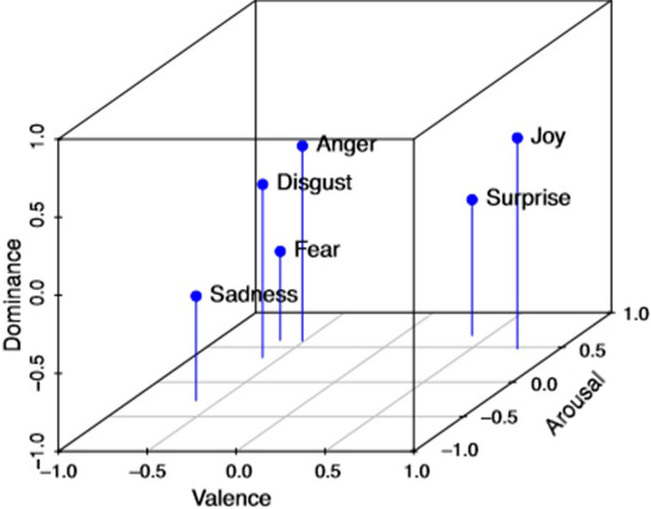
\includegraphics[width=\linewidth]{figs/2_state_of_the_art/VAD_Emotions.jpg}
		\caption{The 3D \acl{vad} model \cite{VAD_Emotions_article}.}
		\label{fig:emoVAD}
	\end{subfigure}
	\caption{Basic emotions spanned across different emotional models.}
\end{figure}


The arousal dimension refers to the level of energy or activation associated with an emotion, or in other words, the strength of the emotion. It measures whether humans are more or less likely to take some action under an emotional state.

The valence dimension measures how a human feels or the nature of the emotion, from positive to negative.

Also, a three-dimensional model may include a dimension of dominance or power, which refers to the seeming strength of the person, or the degree to which an individual feels in control or in charge of the situation that is causing the emotion, usually referred to as \ac{vad} model \cite{RUSSELL1977273}, displayed on figure \ref{fig:emoVAD}.


Dimensional representations of emotions are useful because they provide a wider range of describing an emotional state. Also, they are more suitable for quantifying variations over time, since changing successively from one discrete emotion to another may not make much sense in a real scenario. However, this model isn't as intuitive, therefore, it makes the distinction between a few basic emotions harder, such as surprise, since depending on the context it can have opposite values of valence \cite{Shuman2015}.

\section{Emotion Recognition Datasets}

The quality of the data affects the success of the recognition process. Incomplete, low-quality, or faulty data may lead to incorrect predictions; hence, data should be carefully designed and collected. 

When creating a database for emotion recognition research, researchers must consider factors such as the age, gender, and language of the speakers. Most databases include adult speakers, but there are also databases featuring children and elderly individuals. To improve the representativeness and usefulness of the database, researchers may also consider using different actors to express different emotions.

There are various databases containing emotional expressions in different languages. According to \citeauthor{Scherer2000ACI}, vocal emotion expressions may be driven by universal psychobiological mechanisms, as individuals from diverse cultures and speaking different languages can accurately recognize emotions expressed through speech better than would be expected by chance \cite{Scherer2000ACI}. This is supported by research demonstrating that even infants who cannot yet speak can recognize emotional cues in adult speech \cite{Slaney}. In another study, \citeauthor{Rajoo2016} investigated the influence of language on the ability of a \ac{ser} system, using spoken expressions of four selected emotions (anger, sad, happiness, and neutral) in three languages (Malay, English, and Mandarin). Their study revealed that there are language-specific differences in emotion recognition, with English showing a higher recognition rate compared to Malay and Mandarin. Additionally, the results support the conclusion that \ac{ser} is language-independent, but also suggest that emotions expressed by native speakers are more accurately recognized \cite{Rajoo2016}.

Databases for emotion recognition that can be used have three types:
\begin{itemize}
	\item \textbf{Acted}: recorded by professional or semi-professional actors in sound-proof studios;
	\item \textbf{Elicited}: created by, for example, placing speakers in a simulated emotional situation that can stimulate various emotions;
	\item \textbf{Natural}: mostly obtained from talk shows, call-center recordings, radio talks, and similar sources. Sometimes, these real-world speeches are referred to as spontaneous speech.
\end{itemize}

In video conferencing applications, the conversations take place in natural contexts, which is a fundamental factor to consider when choosing a dataset. Research has demonstrated that there are differences in the characteristics and accuracy of acted and genuine emotions \cite{Vogt}. Some studies have also suggested that simulated emotional speech may not be fully genuine and may be perceived more intensely than genuine emotional speech \cite{2041ade4b5294db59df9f67e9c854632}. Therefore, the studies on emotion recognition have shifted from focusing on induced expressions to spontaneous ones, but data on audiovisual expressions in natural contexts is still limited. Emotion expressions are infrequent, fleeting, and associated with complex contextual structures, making it difficult to collect a large amount of spontaneous data, as shown in a survey on audiovisual emotion recognition \cite{Wu2014}. Ostensibly, different types of databases are suitable for different purposes. For example, a database designed for mainly theoretical research may be more suitable in certain cases rather than one that is intended for use in a real-life industry application.

A summary of prominent datasets and their description is provided in the table \ref{datasets_overview}.

\begin{table}[h]
	\caption{Summary and description of emotion recognition datasets.}
	\centering
	\label{datasets_overview}
	\resizebox{\textwidth}{!}{%
		\begin{tabular}{@{}lcccccc@{}}
			\toprule
			\multicolumn{1}{c}{Dataset} & Format & Language & Content & Emotions & Type\\
			\midrule
			
			\begin{tabular}[c]{@{}c@{}}EMO-DB \cite{Burkhardt2005}\end{tabular} &
			\begin{tabular}[c]{@{}c@{}}Audio\end{tabular} &
			\begin{tabular}[c]{@{}c@{}}German\end{tabular} &
			\begin{tabular}[c]{@{}c@{}}800 recording spoken\\by 10 actors (5 males\\and 5 females).\end{tabular} &
			\begin{tabular}[c]{@{}c@{}}7 emotions: anger, neutral,\\fear, boredom, happiness,\\sadness, disgust.\end{tabular} &
			\begin{tabular}[c]{@{}c@{}}Acted\end{tabular}\\
			
			\begin{tabular}[c]{@{}c@{}}eNTERFACE’05 \cite{Martin2006}\end{tabular} &
			\begin{tabular}[c]{@{}c@{}}Audio\\Video\end{tabular} &
			\begin{tabular}[c]{@{}c@{}}English\end{tabular} &
			\begin{tabular}[c]{@{}c@{}}Videos by 42 subjects,\\coming from 14\\different nationalities.\end{tabular} &
			\begin{tabular}[c]{@{}c@{}}6 emotions: anger, fear,\\surprise, happiness,\\sadness and disgust.\end{tabular} &
			\begin{tabular}[c]{@{}c@{}}Elicited\end{tabular}\\
			
			\begin{tabular}[c]{@{}c@{}}\acs{iemo} \cite{Busso2008}\end{tabular} &
			\begin{tabular}[c]{@{}c@{}}Audio\\Video\\Text\end{tabular} &
			\begin{tabular}[c]{@{}c@{}}English\end{tabular} &
			\begin{tabular}[c]{@{}c@{}}Conversations among\\pairs of 10
				speakers\\(gender balanced)\\spanning 12 hours.\end{tabular} &
			\begin{tabular}[c]{@{}c@{}}10 categorical emotions\\\&  \acs{vad}\end{tabular} &
			\begin{tabular}[c]{@{}c@{}}Acted \&\\Elicited\end{tabular}\\
			
			\begin{tabular}[c]{@{}c@{}}MOUD \cite{moud}\end{tabular} & 
			\begin{tabular}[c]{@{}c@{}}Audio\\Video\end{tabular} &
			\begin{tabular}[c]{@{}c@{}}Spanish\end{tabular} &
			\begin{tabular}[c]{@{}c@{}}80 product reviews\\YouTube videos.\end{tabular} &
			\begin{tabular}[c]{@{}c@{}}Positive, negative, or neutral\\sentiment.\end{tabular} &
			\begin{tabular}[c]{@{}c@{}}Natural\end{tabular}\\
			
			\begin{tabular}[c]{@{}c@{}}CREMA-D \cite{Cao2014}\end{tabular} & 
			\begin{tabular}[c]{@{}c@{}}Audio\\Video\\Text\end{tabular} &
			\begin{tabular}[c]{@{}c@{}}English\end{tabular} &
			\begin{tabular}[c]{@{}c@{}}7442 clips of 12\\sentences spoken by 91\\actors (gender balanced).\end{tabular} &
			\begin{tabular}[c]{@{}c@{}}6 emotions: angry,\\disgusted, fearful, happy,\\neutral, and sad.\end{tabular} &
			\begin{tabular}[c]{@{}c@{}}Acted\end{tabular}\\
			
			\begin{tabular}[c]{@{}c@{}}CMU-MOSI \cite{cmu-mosi}\end{tabular} &
			\begin{tabular}[c]{@{}c@{}}Audio\\Video\end{tabular} &
			\begin{tabular}[c]{@{}c@{}}English\end{tabular} &
			\begin{tabular}[c]{@{}c@{}}2199 movie reviews\\with annotated sentiment.\end{tabular} &
			\begin{tabular}[c]{@{}c@{}}Very negative to very positive\\in seven Likert steps.\end{tabular} &
			\begin{tabular}[c]{@{}c@{}}Natural\end{tabular}\\
			
			\begin{tabular}[c]{@{}c@{}}MSP-Improv \cite{Busso2017}\end{tabular} &
			\begin{tabular}[c]{@{}c@{}}Audio\\Video\\Text\end{tabular} &
			\begin{tabular}[c]{@{}c@{}}English\end{tabular} &
			\begin{tabular}[c]{@{}c@{}}8438 recordings by\\12 actors.\end{tabular} &
			\begin{tabular}[c]{@{}c@{}}4 emotions: angry, sad,\\happy, neutral.\end{tabular} &
			\begin{tabular}[c]{@{}c@{}}Elicited\end{tabular}\\
			
			\begin{tabular}[c]{@{}c@{}}CMU-MOSEI \cite{cmu-mosei}\end{tabular} &
			\begin{tabular}[c]{@{}c@{}}Audio\\Video\\Text\end{tabular} &
			\begin{tabular}[c]{@{}c@{}}English\end{tabular} &
			\begin{tabular}[c]{@{}c@{}}65 hours of YouTube videos\\from more than 1000\\speakers (gender balanced)\\and 250 topics.\end{tabular} &
			\begin{tabular}[c]{@{}c@{}}6 emotions: happiness,\\ sadness, anger, fear,\\disgust, surprise. Polarity\\in Likert scale.\end{tabular} &
			\begin{tabular}[c]{@{}c@{}}Natural\end{tabular}\\
			
			\begin{tabular}[c]{@{}c@{}}MELD \cite{meld}\end{tabular} &
			\begin{tabular}[c]{@{}c@{}}Audio\\Video\\Text\end{tabular} &
			\begin{tabular}[c]{@{}c@{}}English\end{tabular} &
			\begin{tabular}[c]{@{}c@{}}1400 dialogues and 14000\\utterances from Friends\\TV series by multiple\\ speakers.\end{tabular} &
			\begin{tabular}[c]{@{}c@{}}7 emotions: Anger, disgust,\\sadness, joy, neutral, surprise\\and fear. Also positive,\\negative and neutral.\end{tabular} &
			\begin{tabular}[c]{@{}c@{}}Acted\end{tabular}\\
			
			\begin{tabular}[c]{@{}c@{}}RAVDESS \cite{ravdess}\end{tabular} &
			\begin{tabular}[c]{@{}c@{}}Audio\\Video\end{tabular} &
			\begin{tabular}[c]{@{}c@{}}English\end{tabular} &
			\begin{tabular}[c]{@{}c@{}}7356 recordings\\by 24 actors with\\2 statements only.\end{tabular} &
			\begin{tabular}[c]{@{}c@{}}7 emotions: calm, happy,\\sad, angry, fearful,\\surprise, and disgust.\end{tabular} &
			\begin{tabular}[c]{@{}c@{}}Acted\end{tabular}\\
			
			\begin{tabular}[c]{@{}c@{}}MSP-Podcast \cite{Lotfian2019}\end{tabular} &
			\begin{tabular}[c]{@{}c@{}}Audio\end{tabular} &
			\begin{tabular}[c]{@{}c@{}}English\end{tabular} &
			\begin{tabular}[c]{@{}c@{}}100 hours by\\over 100 speakers\end{tabular} &
			\begin{tabular}[c]{@{}c@{}}Activation, dominance and\\valence and 9\\categorical labels\end{tabular} &
			\begin{tabular}[c]{@{}c@{}}Natural\end{tabular}\\
			
			\begin{tabular}[c]{@{}c@{}}TESS \cite{tess}\end{tabular} &
			\begin{tabular}[c]{@{}c@{}}Audio\end{tabular} &
			\begin{tabular}[c]{@{}c@{}}English\end{tabular} &
			\begin{tabular}[c]{@{}c@{}}2800 recording by\\2 actresses.\end{tabular} &
			\begin{tabular}[c]{@{}c@{}}7 emotions: anger, disgust,\\fear, happiness, pleasant\\surprise, sadness, and neutral.\end{tabular} &
			\begin{tabular}[c]{@{}c@{}}Acted\end{tabular}\\
			
			\bottomrule
		\end{tabular}%
} \end{table}

In a \citeyear{Jahangir2021} \ac{ser} \ac{sota} review article, \citeauthor{Jahangir2021} exhibited the most commonly used databases in their selected studies, figure \ref{fig:databases} \cite{Jahangir2021}. They realized the most popular ones had a gender-balanced number of speakers with high-quality recordings.

\begin{figure}[h]
	\centering
	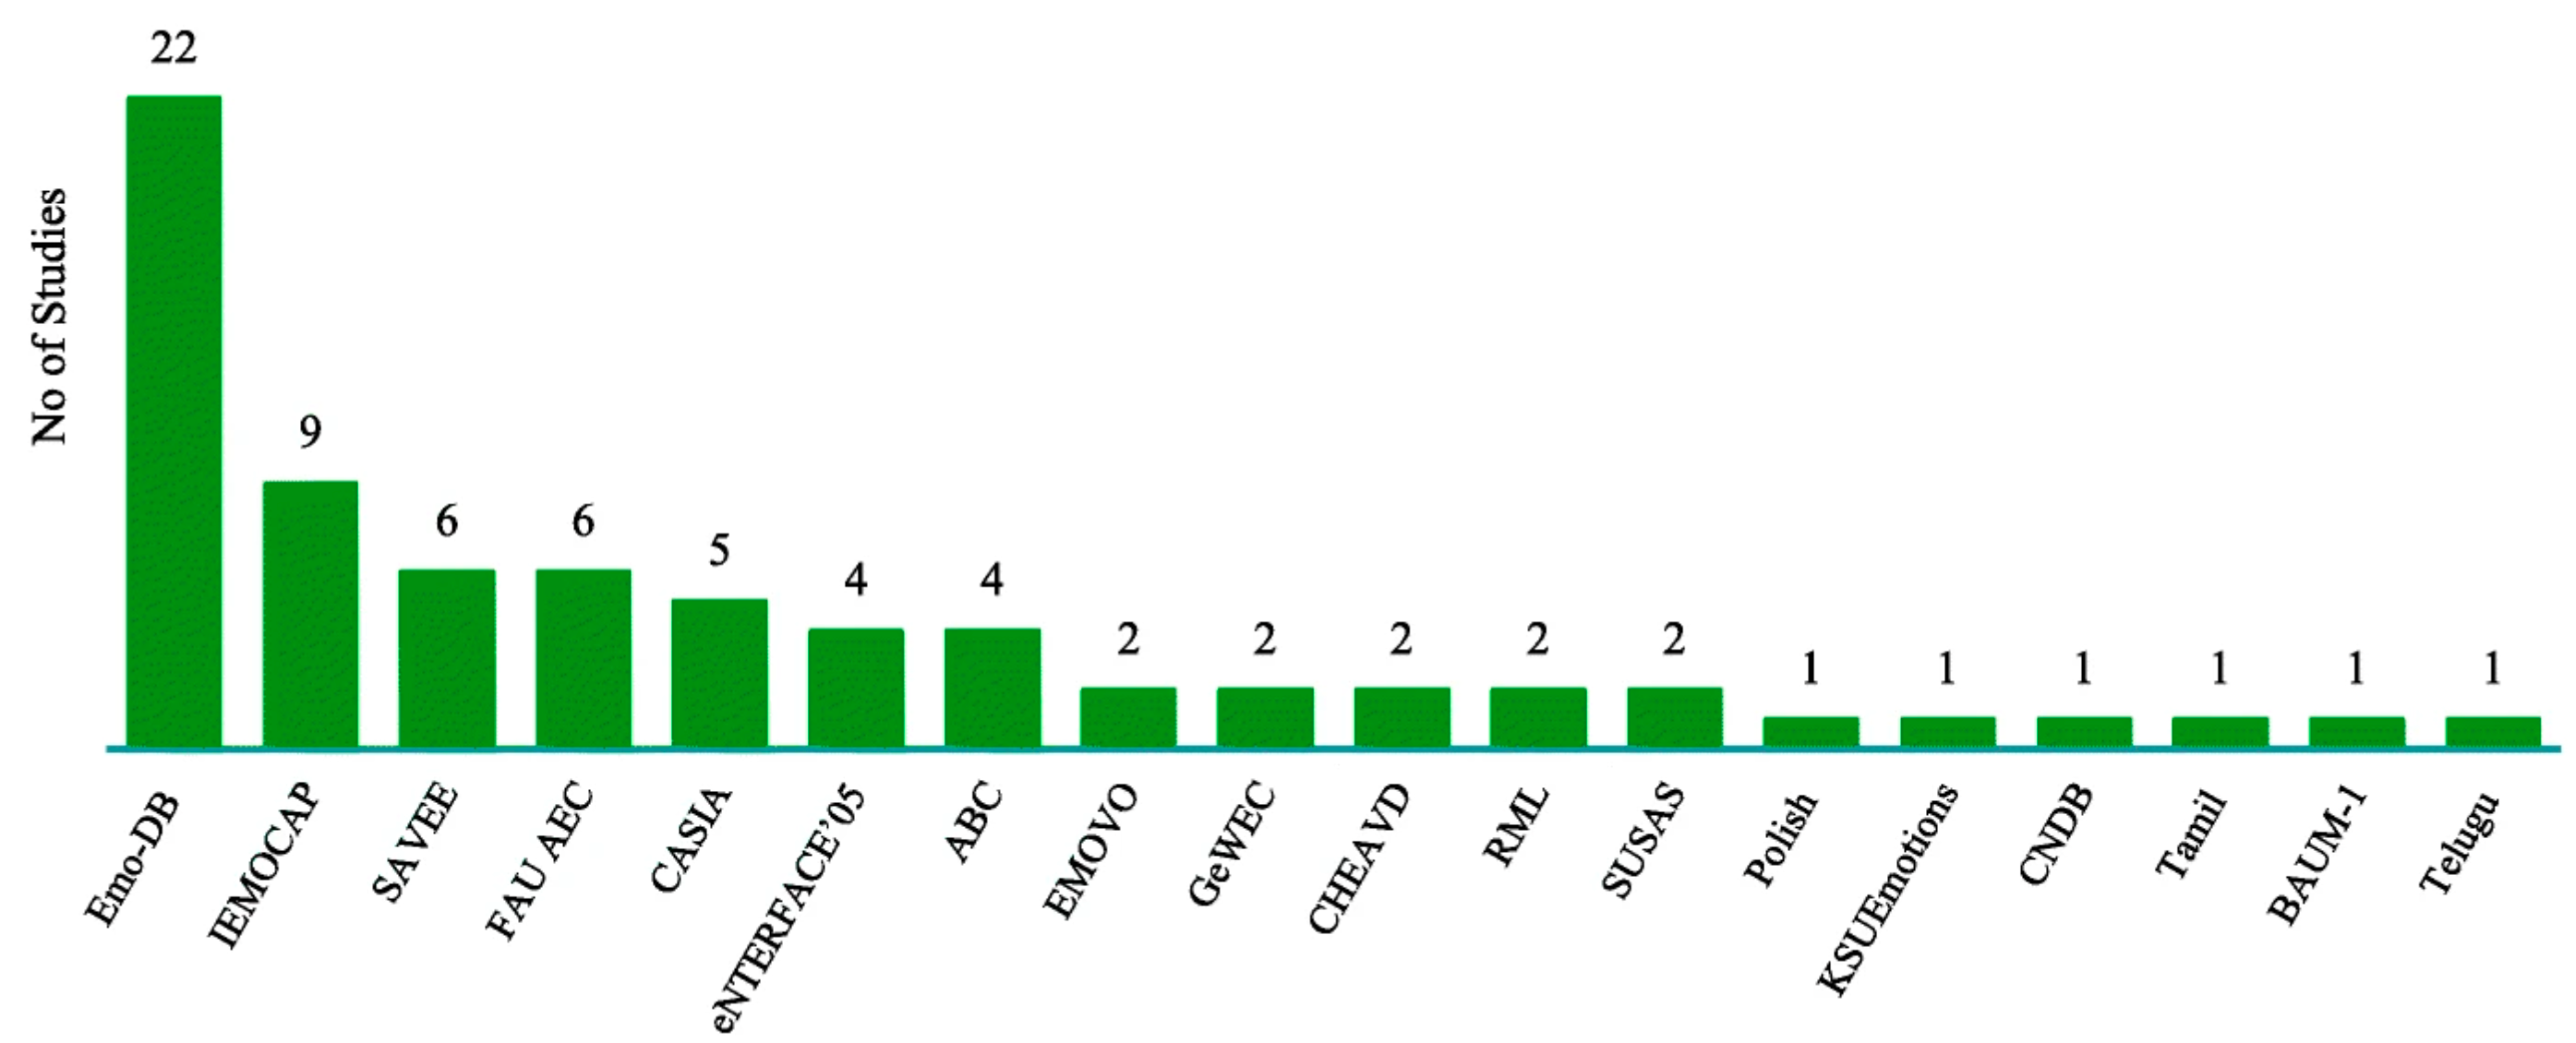
\includegraphics[width=\linewidth]{figs/2_state_of_the_art/sota.png}
	\caption{Frequency distribution of databases on reviewed articles from a \ac{sota} study \cite{Jahangir2021}.}
	\label{fig:databases}
\end{figure}

\section{\acl{ser}}

\ac{ser} is a subfield of artificial intelligence that focuses on the development of systems that can identify and classify the emotional state of a speaker based on their speech.

Speech is a vital tool for human communication and social interaction. Fundamentally, it is a continuous signal that can convey information, express emotions, and share meaning \cite{Narayanan2013}.

Words alone do not always transmit sufficient emotion, for instance, text messages can be easily misconceived. Hence, the necessity of \ac{ser} to aid and complete this task of figuring out the emotions/intent of human interaction. 

\subsection{Speech Features}

Speech features are characteristics of an audio signal that can be extracted and analyzed to understand its properties. These features are commonly categorized into the following three classes:
\begin{itemize}
	\item \textbf{Prosodic Features};
	\item \textbf{Spectral Features};
	\item \textbf{Voice Quality Features}.
\end{itemize}

Prosodic and spectral features are commonly employed in various fields, as they have been shown to effectively improve outcomes. By combining these features, it is possible to further optimize their usefulness and attain even better results.

Currently, there are a wide variety of acoustic properties that can be used to extract a large feature vector. Examples of these features include pitch, intensity, duration, and voice quality, which then several common statistics can be applied to them, such as minimum, mean, maximum, etc., as shown in table \ref{tab:features} adapted from a book \cite{Schuller2011}.


\begin{table}[h]
	\centering
	\caption{Overview on features commonly used for acoustic emotion recognition \cite{Schuller2011}.}
	\label{tab:features}
	\resizebox{\textwidth}{!}{%
		\begin{tabular}{lllllll}
			\hline
			\multicolumn{1}{|l|}{\begin{tabular}[c]{@{}l@{}}\textbf{Intonation}\\ (F0 or pitch modelling)\end{tabular}} &
			\multicolumn{1}{l|}{} &
			\multicolumn{1}{l|}{} &
			\multicolumn{1}{l|}{} &
			\multicolumn{1}{l|}{\begin{tabular}[c]{@{}l@{}}\textbf{Extremes}\\ (min, max, range, ...)\end{tabular}} &
			\multicolumn{1}{l|}{} &
			\multicolumn{1}{l|}{} \\ \cline{1-1} \cline{5-5}
			\multicolumn{1}{|l|}{\begin{tabular}[c]{@{}l@{}}\textbf{Intensity}\\ (energy, Teager, ...)\end{tabular}} &
			\multicolumn{1}{l|}{} &
			\multicolumn{1}{l|}{} &
			\multicolumn{1}{l|}{} &
			\multicolumn{1}{l|}{\begin{tabular}[c]{@{}l@{}}\textbf{Mean}\\ (arithmetic, absolute, ...)\end{tabular}} &
			\multicolumn{1}{l|}{} &
			\multicolumn{1}{l|}{} \\ \cline{1-1} \cline{5-5}
			\multicolumn{1}{|l|}{\begin{tabular}[c]{@{}l@{}}\textbf{Linear Prediction}\\ (LPCC, PLP, ...)\end{tabular}} & \multicolumn{1}{l|}{\multirow{9}{*}{\begin{tabular}[c]{@{}l@{}}\textbf{Deriving}\\ (raw LLD, \\ deltas, \\ regression \\ coefficients, \\ LDA, \\ PCA, ...)\end{tabular}}} &
			\multicolumn{1}{l|}{\multirow{9}{*}{\begin{tabular}[c]{@{}l@{}}\textbf{Filtering}\\ (smoothing,\\ normalizing,\\ ...)\end{tabular}}} &
			\multicolumn{1}{l|}{\multirow{9}{*}{\begin{tabular}[c]{@{}l@{}}\textbf{Chunking}\\ (absolute,\\ relative,\\ ...)\end{tabular}}} &
			\multicolumn{1}{l|}{\begin{tabular}[c]{@{}l@{}}\textbf{Percentiles}\\ (quartiles, ranges, ...)\end{tabular}} & \multicolumn{1}{l|}{\multirow{9}{*}{\begin{tabular}[c]{@{}l@{}}\textbf{Deriving}\\ (raw LLD, \\ deltas, \\ regression \\ coefficients, \\ LDA, \\ PCA, ...)\end{tabular}}} &
			\multicolumn{1}{l|}{\multirow{9}{*}{\begin{tabular}[c]{@{}l@{}}\textbf{Filtering}\\ (smoothing,\\ normalizing,\\ ...)\end{tabular}}} \\ \cline{1-1} \cline{5-5}
			\multicolumn{1}{|l|}{\begin{tabular}[c]{@{}l@{}}\textbf{Cepstral Coefficients}\\ (MFCC, ...)\end{tabular}} &
			\multicolumn{1}{l|}{} &
			\multicolumn{1}{l|}{} &
			\multicolumn{1}{l|}{} &
			\multicolumn{1}{l|}{\begin{tabular}[c]{@{}l@{}}\textbf{Higher Moments}\\ (std. dev., kurtosis, ...)\end{tabular}} &
			\multicolumn{1}{l|}{} &
			\multicolumn{1}{l|}{} \\ \cline{1-1} \cline{5-5}
			\multicolumn{1}{|l|}{\begin{tabular}[c]{@{}l@{}}\textbf{Formants}\\ (amplitude, position, ...)\end{tabular}} &
			\multicolumn{1}{l|}{} &
			\multicolumn{1}{l|}{} &
			\multicolumn{1}{l|}{} &
			\multicolumn{1}{l|}{\begin{tabular}[c]{@{}l@{}}\textbf{Peaks}\\ (number, distances, ...)\end{tabular}} &
			\multicolumn{1}{l|}{} &
			\multicolumn{1}{l|}{} \\ \cline{1-1} \cline{5-5}
			\multicolumn{1}{|l|}{\begin{tabular}[c]{@{}l@{}}\textbf{Spectrum}\\ (MFB, NMF, roll-off, ...)\end{tabular}} &
			\multicolumn{1}{l|}{} &
			\multicolumn{1}{l|}{} &
			\multicolumn{1}{l|}{} &
			\multicolumn{1}{l|}{\begin{tabular}[c]{@{}l@{}}\textbf{Segments}\\ (number, duration, ...)\end{tabular}} &
			\multicolumn{1}{l|}{} &
			\multicolumn{1}{l|}{} \\ \cline{1-1} \cline{5-5}
			\multicolumn{1}{|l|}{\begin{tabular}[c]{@{}l@{}}\textbf{TF-Transformation}\\ (Wavelets, Gabor, ...)\end{tabular}} &
			\multicolumn{1}{l|}{} &
			\multicolumn{1}{l|}{} &
			\multicolumn{1}{l|}{} &
			\multicolumn{1}{l|}{\begin{tabular}[c]{@{}l@{}}\textbf{Regression}\\ (coefficients, error, ...)\end{tabular}} &
			\multicolumn{1}{l|}{} &
			\multicolumn{1}{l|}{} \\ \cline{1-1} \cline{5-5}
			\multicolumn{1}{|l|}{\begin{tabular}[c]{@{}l@{}}\textbf{Harmonicity}\\ (HNR, spectral tilt, ...)\end{tabular}} &
			\multicolumn{1}{l|}{} &
			\multicolumn{1}{l|}{} &
			\multicolumn{1}{l|}{} &
			\multicolumn{1}{l|}{\begin{tabular}[c]{@{}l@{}}\textbf{Spectral}\\ (DCT coefficients, ...)\end{tabular}} &
			\multicolumn{1}{l|}{} &
			\multicolumn{1}{l|}{} \\ \cline{1-1} \cline{5-5}
			\multicolumn{1}{|l|}{\begin{tabular}[c]{@{}l@{}}\textbf{Perturbation}\\ (jitter, shimmer, ...)\end{tabular}} &
			\multicolumn{1}{l|}{} &
			\multicolumn{1}{l|}{} &
			\multicolumn{1}{l|}{} &
			\multicolumn{1}{l|}{\begin{tabular}[c]{@{}l@{}}\textbf{Temporal}\\ (durations, positions,  ...)\end{tabular}} &
			\multicolumn{1}{l|}{} &
			\multicolumn{1}{l|}{} \\ \hline
			\\
			\multicolumn{4}{l}{\textbf{Low-Level-Descriptors}} &
			\multicolumn{3}{l}{\textbf{Functionals}}
		\end{tabular}%
	}
\end{table}


\subsubsection{Prosodic Features}

Prosodic features are those that can be perceived by humans, such as intonation, rhythm, and loudness. The most widely used ones are based on \textbf{pitch}, \textbf{energy}, and \textbf{duration}.

Pitch, also known as the fundamental frequency or F0, refers to the lowest frequency of a periodic waveform. It is often used to convey emotion because it is influenced by the tension in the vocal folds and the sub-glottal air pressure. Studies have shown that the average pitch for males is typically about an octave lower than that of females, with an average pitch of 120 Hertz for males, 229 Hertz for females, and 155–185 Hertz for those with ambiguous gender. According to the study conducted by \citeauthor{ArputhaRathina2012} in \citeyear{ArputhaRathina2012}, there are clear differences in the pitch of the female and male genders when expressing different emotions. These differences may present a challenge for a gender-independent emotion classifier that relies solely on pitch \cite{ArputhaRathina2012}.

\begin{figure}[h]
	\centering
	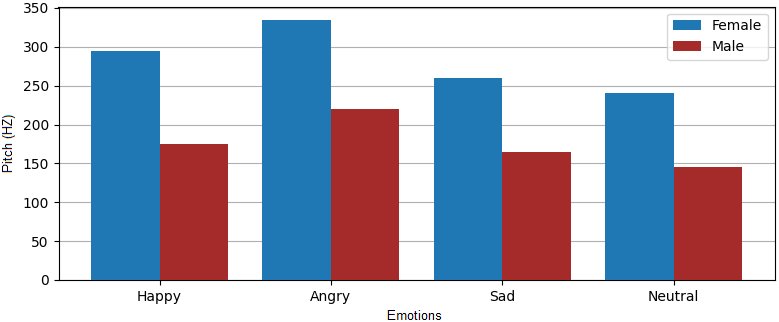
\includegraphics[width=.8\linewidth]{figs/2_state_of_the_art/Average-Pitch-Comparison-of-Male-and-Female-speak-ers.png}
	\caption{Average pitch comparison of male and female speakers’ \cite{ArputhaRathina2012}.}
	\label{fig:avgpitch}
\end{figure}

Prosodic features have been indicated as the most distinctive properties of emotional content for speech emotion recognition \cite{ZhihongZeng2009}.

\subsubsection{Spectral Features}

In the field of speech and audio processing, spectral features are used to analyze the characteristics of the human voice, which can convey information such as emotion, identity, and speaker traits.  The spectral content of speech signals varies significantly depending on the sounds being produced and the language being spoken, and it is often highly dynamic and time-varying.

One commonly used spectral feature is the \ac{mfccs}. \ac{mfccs} are calculated by performing a \ac{ft} on a window of audio data to obtain the spectral power, which is then mapped to the Mel-scale (a frequency scale that reflects how the human auditory system perceives sound). The Mel-scaled spectral power is then transformed into the cepstral domain using a discrete cosine transform, resulting in the \ac{mfccs} that represent the spectral power of the signal in the cepstral domain and can be used as input for tasks such as emotion recognition.

Another spectral feature is the gammatone frequency cepstral coefficient, which is similar to \ac{mfccs} in that they are derived using a \ac{ft} and a filter bank (in this case, a gammatone filter bank that models the auditory system's response to different frequencies). Linear prediction cepstral coefficients are another type of feature that is derived from the linear prediction of a signal. Log-frequency power coefficients are a type of feature that mimic the logarithmic filtering characteristics of the human auditory system and are obtained by measuring spectral band energies using a fast Fourier transform. 


\subsubsection{Voice Quality Features}

Voice quality is the set of characteristics that distinguish one person's voice from another. Some common methods for analyzing voice quality involve examining the physical properties of the vocal tract, such as jitter, shimmer, and the harmonics-to-noise ratio.

These properties may change involuntarily and can be used to differentiate emotions in the speech signal. Jitter refers to the variability in the period, or the time between successive peaks, of the fundamental frequency, whereas shimmer refers to the variability in the amplitude. The harmonics-to-noise ratio is a measure of the relative strength of the harmonics in a speech signal compared to the noise.

These three measures are often used together to assess the quality of a person's voice and can be useful in several tasks, e.g., treatment of voice disorders, age detection, speaker or emotion recognition, etc.

\subsection{Strategies}

The use case for this specific system of \ac{ser} is a video conferencing application where conversations are unpredictable, therefore, it is necessary to have a robust speech recognition system, however, some approaches can create privacy issues, for users who may not want to have their private conversations public, and even, ethical issues. Therefore, combining acoustic and linguistic content, by transcribing the speech to text, was not intended in this work, nonetheless, it is a remarkable approach that would potentially improve the system.

A \ac{ser} system requires a large and diverse dataset of speech samples, as well as feature extraction and preprocessing techniques to obtain relevant features from the audio signal, such as the ones mentioned above. Appropriate machine learning algorithms are then used to classify the emotional content of the speech based on the extracted features. In the past several years, classical machine learning algorithms, such as \ac{hmm} \cite{1220939}, \ac{svm}, and decision tree-based methods, have been utilized for audio sentiment analysis. More recently, researchers have proposed various neural network-based architectures to improve audio sentiment analysis. With the development of \ac{dl}, more complex neural-based architectures are proposed. For example, \ac{cnn}-based models have been used to train with the audio spectrograms or features derived from the signal.

Currently, there are two main types of implementations \cite{Zhao2018}:
\begin{itemize}
	\item \textbf{The traditional feature-based \ac{ser}}: hand-crafted features are extracted by applying a series of statistical aggregation functions to acoustic features of the audio signal, which are then passed on to a classifier;
	\item \textbf{Automatic feature extraction-based \ac{ser}}: avoids manual feature engineering and leverages the abilities of \ac{dl} techniques. This method typically involves using raw speech signals, Mel spectrograms, or \ac{mfccs} as input for a \ac{dnn} model.
\end{itemize}


\begin{figure}[h]
	\centering
	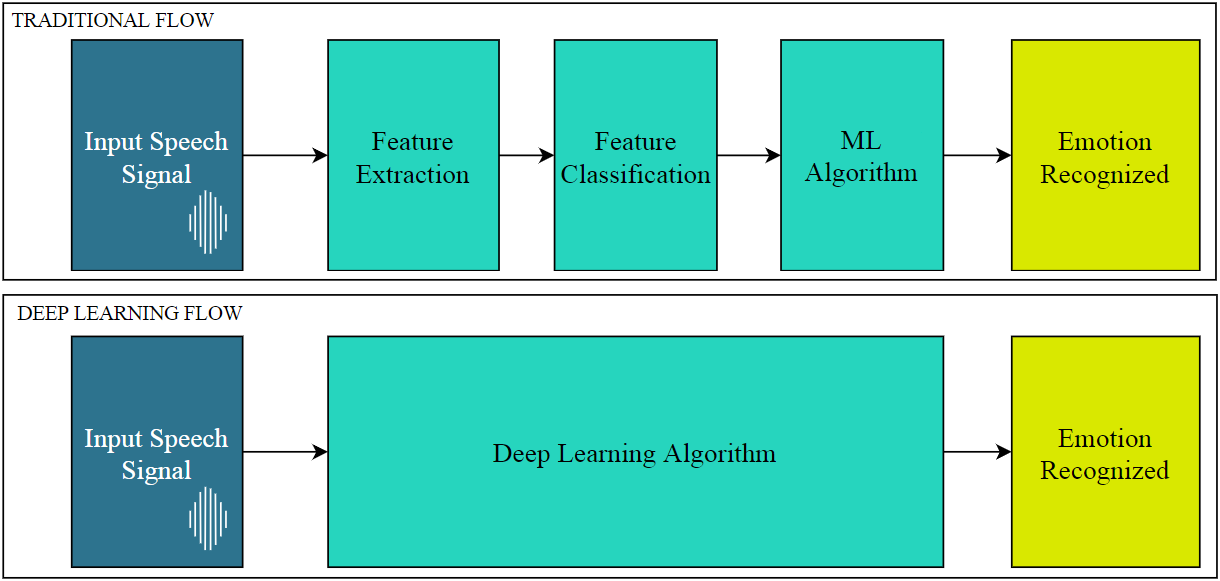
\includegraphics[width=\linewidth]{figs/2_state_of_the_art/methods.png}
	\caption{Traditional machine learning flow vs. automatic feature extraction with \ac{dl} flow \cite{Khalil2019}.}
	\label{fig:methods}
\end{figure}

Figure \ref{fig:methods}, displays the main difference between the methods, the traditional implementation has more steps because it mainly depends on the feature extraction and selection processes. The \ac{dl} approaches avoid feature engineering and tend to improve recognition efficiency, however, it significantly increases complexity and the computational cost, which has a negative effect on \ac{ser} systems used in real-time scenarios.

\subsection{Traditional Feature-Based \ac{ser}}

The traditional feature-based \ac{ser} is a challenging task for researchers. It consists of applying a series of statistical aggregation functions (e.g., mean, max, variance, etc.) on acoustic features extracted from the speech to produce a statistical feature vector. The feature vector obtained can describe the temporal variations of speech signals, which are considered to be associated with the subjacent emotion. This vector is then analyzed, and feature selection is performed on it to reduce its size and reduce overfitting to the data, and finally, various classifiers are given that vector as input and are evaluated to find the most suitable for the task.

In \ac{sota} articles, the final set of selected features is often not the same across different studies. This selection of features for training classifiers has a significant impact on the overall performance of the \ac{ser} system, which is why it is a major challenge.

The statistical feature vector may contain only global features, extracted from the full-length utterance, or several local features, extracted from speech segments obtained from framing the utterance. The performance of the features based on their granularity is also analyzed in several studies.

\citeauthor{1202279} found that using global features (computed from gross statistics) resulted in a recognition rate of 86.6\% while using local features (computed from syllable duration, pitch, and energy values) resulted in a recognition rate of 77.6\%, while human judges had a recognition rate of 79.8\% \cite{1202279}. In a separate study, \citeauthor{Rao2012} observed that combining local and global prosodic features slightly improved performance compared to using only local features \cite{Rao2012}.


Forward methods and backward methods are two common techniques for feature selection. Forward methods begin with an empty (or very limited) feature set and add features incrementally. The most well-known forward method is the Sequential Forward Selection algorithm, which at each step tries adding each feature to the set and keeps the one that results in the highest improvement in accuracy.

\citeauthor{Luengo2005} (\citeyear{Luengo2005}) applied a Forward 3-Backward 1 wrapper method to select features. This method involves choosing the feature that maximizes accuracy in each step using leave-one-out testing. After three consecutive selections, the least useful feature is eliminated. Without feature selection, the authors obtained a recognition rate of 93.50\% with a \ac{svm} classifier and 84.79\% with a Gaussian Mixture Model using 86 prosodic features. However, by using the selected six best features, the recognition rates changed to 92.38\% and 86.71\%. In conclusion, it was noted that a slight reduction in recognition rate is compensated by a much lower computational cost of extracting and training the features.

In \citeyear{Gosztolya2015}, \citeauthor{Gosztolya2015} demonstrated that classification and regression algorithms can benefit from even simple feature selection techniques. They proposed a simple greedy forward-backward feature selection algorithm, which is less computationally costly than any other methods, for speech conflict intensity estimation, which significantly outperformed previous scores \cite{Gosztolya2015}.


\ac{cfs} is another popular method used in machine learning and data mining. \ac{cfs} involves calculating the correlation between each feature and the target variable, ranking the features based on their correlations, and selecting a subset of the highest-ranked features for use in a model. The goal of \ac{cfs} is to select a subset of features that are highly correlated with the target variable and not highly correlated with each other, to improve the performance of the model and reduce overfitting. In a study by \citeauthor{Schuller3D2011}, this method was applied to reduce the number of acoustic features from 760, for each of valence, activation, and dominance dimensions, to 238, 109, and 88, respectively, and improved their results by doing so \cite{Schuller3D2011}.

The \ac{gemaps} is a set of features used in speech emotion recognition developed by researchers at the University of Geneva \cite{Eyben2016}. It is designed to be a compact and efficient feature set for automatic emotion recognition from speech. It includes a range of prosodic and acoustic features that are relevant to emotion recognition, such as pitch, intensity, spectral properties, and temporal features. \ac{gemaps} feature set has been utilized in several studies on speech emotion recognition, e.g., \cite{Tarantino2019}, as well as in applications such as affective computing, virtual assistants, and human-computer interaction.

Many of the early researchers used traditional machine learning classification techniques such as Linear Discriminant Analysis, Regular Discriminant Analysis, \ac{svm}, K-Nearest Neighbors, \acp{random forest}, and Gaussian Mixture Models \cite{Kuchibhotla2014}. Moreover, ensemble learning has also been employed by researchers to combine the predictions of multiple individual classifiers to improve performance.

\citeauthor{Albornoz2011} built a hierarchical classifier with two stages, on each stage they predicted different emotions using a different set of features and classifiers \cite{Albornoz2011}. They showed that 12 mean \ac{mfccs} features, deltas, and acceleration coefficients are the best features for the first stage with a \ac{hmm} with 30 Gaussians in the mixture classifier. For the second stage with a \ac{hmm}, they obtained as the best features, 12 means \acp{mfccs}, 30 means log-spectrum, and mean and standard deviation pitch. Using the EMO-DB corpus, they achieved an accuracy of 71.75\%.

In a study, \citeauthor{Lee2011} (\citeyear{Lee2011}) used a traditional strategy to extract 16 low-level descriptors from audio data, including zero crossing rate, root-mean-square energy, pitch, harmonics-to-noise ratio, and 12 \ac{mfccs} and deltas. They then applied 12 different statistical functions, resulting in a set of 384 acoustic features per utterance. The researchers used a multi-level binary decision tree structure with different classifiers at each level to classify the data by dividing the problem into sub-problems. For example, at the first level, they compared the "neutral" label to all other labels. This approach resulted in an \ac{uar} of 41.57\% on the AIBO dataset and 58.46\% on the \ac{iemo} dataset \cite{Lee2011}, with 5 and 4 classes respectively.

In \citeyear{HandCraftedSahu}, \citeauthor{HandCraftedSahu} developed a set of hand-crafted features for an audio signal using the \ac{iemo} dataset. The authors obtained an eight-dimensional vector by applying statistical functions to acoustic features such as pitch, harmonics, and pause \cite{HandCraftedSahu}. They also found that ensembling models improved performance, and they achieved a maximum accuracy of 56.6\% with a model that combined \ac{rf}, \ac{xgb}, and a multilayer perceptron.

A new architecture was introduced in \citeyear{Issa2020} by \citeauthor{Issa2020}, for identifying emotions in sound files using a one-dimensional \ac{cnn}, which is not typically considered a traditional model, however the extraction of features was still performed manually. They obtain a one-dimensional array by taking mean values along the time axis of 193 features, including \ac{mfccs}, chromagram, Mel spectrogram, Tonnetz representation, and spectral contrast, from the sound files and use them as inputs for the \ac{cnn}. The proposed framework was evaluated using samples from the RAVDESS, EMO-DB, and \ac{iemo} datasets. The framework achieved accuracies of 71.61\% for RAVDESS (with 8 emotions), 86.1\% for EMO-DB (with 7 emotions), 95.71\% for EMO-DB (with 7 emotions), and 64.3\% for \ac{iemo} (with 4 emotions) in speaker-independent audio classification tasks \cite{Issa2020}.

\subsection{\acl{dl}-Based \ac{ser}}

As \ac{dl} technology has advanced, automatic feature learning algorithms have become increasingly popular for \ac{ser}, and even in other areas, for example, in cardiac spectrogram analysis, it is one of the state-of-art approaches, \cite{8759878} and \cite{Zhou2022}, in which the spectrogram of the audio from the heartbeat is used to evaluate the cardiac activity. These algorithms are effective at learning task-specific features without the need for extensive manual feature engineering.

\ac{dnn} techniques for \ac{ser} are primarily trained using raw signals, spectrograms, low-level descriptors, and \ac{mfccs}, which have been shown to produce satisfactory results. Various \ac{dnn} architectures including \ac{rnn}, \ac{lstm}, and attention-based convolution \ac{rnn} have been designed for \ac{ser}, each with its strengths and weaknesses. \acp{cnn} and their variations are the most common, as they are known for their ability to extract a large number of hidden features from signals and images. It is also important to note that the way the information contained in an audio spectrogram is used can be different, as some authors use three channels of the spectrogram, such as the RGB of the plotted image, or even using the static, delta, and delta-deltas of it, essentially having a 3-D tensor, while other authors use a 2-D tensor with the numeric spectrogram values.

In a paper published in \citeyear{GARCIAORDAS2021102946}, \citeauthor{GARCIAORDAS2021102946} proposed a fully \ac{cnn} that can process variable input lengths for near real-time sentiment analysis \cite{GARCIAORDAS2021102946}. The use of \acp{mfccs} made it easier to identify emotions in audio signals. The model achieved superior performance compared to other machine learning models on the EmoDB, RAVDESS, and TESS datasets, with accuracies of 75.28\%, 92.71\%, and 99.03\%, respectively.

The use of \acp{cnn} and \acp{rnn} increased in recent years, driven by their successes in various applications, and researchers have begun exploring the potential benefits of combining these models into a single architecture. For example, in a previous study, \citeauthor{ma18b_interspeech} (\citeyear{ma18b_interspeech}) proposed a neural network architecture designed specifically to handle variable-length speech by combining \ac{cnn}-based deep spectrogram representations with a \ac{rnn} to process variable-length speech segments. Their model achieved a weighted and unweighted accuracy of 71.4\% and 64.22\% on the \ac{iemo} dataset \cite{ma18b_interspeech}. In another study that used the same corpus, \citeauthor{Zhao2019} (\citeyear{Zhao2019}) developed an attention-based bidirectional \ac{lstm} \ac{rnn} with attention-based fully convolutional networks and achieved weighted and unweighted accuracies of 68.1\% and 67.0\% \cite{Zhao2019}.

\citeauthor{Luo2018} in \citeyear{Luo2018}, proposed a model for audio sentiment analysis that combines multiple traditional acoustic features and spectrum graphs. The authors analyze the \ac{mfccs}, spectral centroid, chroma-short-time \ac{ft}, and spectral contrast. The best model used is a combination of a \ac{lstm} network and a \ac{cnn}. The model was tested on the CMU-MOSI and MOUD datasets, achieving accuracies of 68.74\% and 69.64\% for 4 and 2 emotion classes, respectively.

In \citeyear{8421023}, \citeauthor{8421023} proposed a 3-D attention-based convolutional \ac{rnn}, which learns discriminative features from the input data. The input to the model is a Mel spectrogram with static, deltas, and delta-deltas, which is processed by a 3-D \ac{cnn} and then combined with a \ac{lstm} for high-level feature extraction. To address silent and emotion-irrelevant frames, an additional attention model is used to focus on emotion-relevant frames and produce discriminative utterance-level features. Their proposed method achieved \ac{sota} performance on the \ac{iemo} and Emo-DB corpora, with \acp{uar} of 64.74±5.44\% and 82.82±4.99\% \cite{8421023}.

In a paper published by \citeauthor{Muppidi2021}, the authors proposed one of the first quaternion-based \ac{cnn} for \ac{ser}. Their model is significantly smaller than other \ac{dl} models and achieved \ac{sota} results in terms of accuracy on several datasets, including RAVDESS (77.67\% accuracy with 8 emotions), \ac{iemo} (70.46\% accuracy with 4 emotions), and EMO-DB (88.78\% accuracy with 7 emotions) \cite{Muppidi2021}.


\subsubsection{Transfer Learning}

Transfer learning is a machine learning technique that involves using the knowledge gained from training a model on one task to improve the performance of a model on a related task.

As stated before, finding a large amount of labeled data to train a \ac{ser} system can be challenging. That is why leveraging the knowledge gained from training a model on a large dataset of speech samples can be particularly useful to reduce the amount of data and computational cost required.

Although there is a significant difference between audio signals and spectrograms and standard ImageNet images, the principles of transfer learning still apply. In a \citeyear{rethinkPalanisamy} paper, \citeauthor{rethinkPalanisamy} demonstrated this by using pre-trained weights from image classification models led to improved performance compared to using randomly initialized weights. Their ensemble of models pre-trained on ImageNet achieved \ac{sota} results on the ESC-50 and UrbanSound8K datasets \cite{rethinkPalanisamy}.

It is also common to extract features from the spectrogram images using pre-trained models and use them as input to more traditional machine learning models, as shown in a study by \citeauthor{8085174}, that used the pre-trained \ac{cnn} AlexNet model to learn deep features and feed them to a \ac{svm} \cite{8085174}.

In table \ref{tab:article_overview} we provide a list of our reviewed articles for both strategies commonly used in audio classification tasks, and, subsequently, \ac{ser} tasks.

\begin{table}[h]
	\centering
	\caption{Overview of audio classification articles with strategies.}
	\label{tab:article_overview}
	\resizebox{\textwidth}{!}{%
		\begin{tabular}{@{}lccc@{}}
			\toprule
			Paper Title (Publication Date) &
			Audio Features &
			Classifier &
			\begin{tabular}[c]{@{}c@{}}Datasets (N\textsuperscript{\underline{o}} of Labels):\\Accuracy (\%)\end{tabular}\\ 
			
			\toprulec
			\rowcolor{gray!25}
			\multicolumn{4}{c}{Traditional Feature-Based \ac{ser} Approaches} \\
			\midrulec
			
			\addlinespace[2mm]
			
			\begin{tabular}[l]{@{}l@{}}Spoken emotion recognition\\using hierarchical\\classifiers (\citeyear{Albornoz2011}) \cite{Albornoz2011}\end{tabular} &
			\begin{tabular}[c]{@{}c@{}}\ac{mfccs}\\Log-spectrum\\Pitch\end{tabular} &
			\begin{tabular}[c]{@{}c@{}}\ac{hmm}\end{tabular} &
			\begin{tabular}[c]{@{}c@{}}EMO-DB (7): 71.75\end{tabular} \\
			
			\addlinespace[2mm]
			
			\begin{tabular}[l]{@{}l@{}}Emotion recognition\\using a hierarchical\\binary decision\\tree approach\\(\citeyear{Lee2011}) \cite{Lee2011}\end{tabular} &
			\begin{tabular}[c]{@{}c@{}}Zero crossing rate\\Root-mean-square energy\\Pitch\\\ac{mfccs}\\Harmonics-to-noise ratio\end{tabular} &
			\begin{tabular}[c]{@{}c@{}}Multi-level binary\\decision trees\end{tabular} &
			\begin{tabular}[c]{@{}c@{}}(\acp{uar})\\AIBO (5): 41.57\\\ac{iemo} (4): 58.46\end{tabular} \\
			
			\addlinespace[2mm]
			
			\begin{tabular}[l]{@{}l@{}}Multimodal \ac{ser}\\and Ambiguity\\Resolution (\citeyear{HandCraftedSahu}) \cite{HandCraftedSahu}\end{tabular} &
			\begin{tabular}[c]{@{}c@{}}Pitch\\Harmonics\\Pause\end{tabular} &
			\begin{tabular}[c]{@{}c@{}}Random forest, extreme\\gradient boosting and\\multilayer perceptron\end{tabular} &
			\begin{tabular}[c]{@{}c@{}}\ac{iemo} (4): 56.6\end{tabular} \\
			
			\addlinespace[2mm]
			
			\begin{tabular}[l]{@{}l@{}}\ac{ser} with deep \acp{cnn}\\(\citeyear{Issa2020}) \cite{Issa2020}\end{tabular} &
			\begin{tabular}[c]{@{}c@{}}\ac{mfccs}\\Chromagram\\Mel spectrogram\\Spectral contrast\end{tabular} &
			\begin{tabular}[c]{@{}c@{}}One-dimensional\\\ac{cnn}\end{tabular} &
			\begin{tabular}[c]{@{}c@{}}RAVDESS (8): 71.61\\ \ac{iemo} (4): 64.30\\ EMO-DB (7): 86.10\end{tabular} \\
			
			\addlinespace[2mm]
			
			\toprulec
			\rowcolor{gray!25}
			\multicolumn{4}{c}{\acl{dl}-Based \ac{ser} Approaches} \\
			\midrulec
			
			\addlinespace[2mm]
			
			\begin{tabular}[l]{@{}l@{}}Sentiment analysis in\\non-fixed length audios\\using a Fully \ac{cnn} (\citeyear{GARCIAORDAS2021102946}) \cite{GARCIAORDAS2021102946}\end{tabular} &
			\begin{tabular}[c]{@{}c@{}}Mel-Spectrogram\\\ac{mfccs}\end{tabular} &
			\begin{tabular}[c]{@{}c@{}}Fully \ac{cnn}\end{tabular} &
			\begin{tabular}[c]{@{}c@{}}RAVDESS (8): 75.28\\EMO-DB (7): 92.71\\TESS: 99.03\end{tabular} \\
			
			\addlinespace[2mm]
			
			\begin{tabular}[l]{@{}l@{}}Emotion Recognition from\\Variable-Length Speech\\Segments Using \ac{dl}\\on Spectrograms (\citeyear{ma18b_interspeech}) \cite{ma18b_interspeech}\end{tabular} &
			\begin{tabular}[c]{@{}c@{}}Log-Spectrograms\end{tabular} &
			\begin{tabular}[c]{@{}c@{}}\ac{cnn} and \ac{rnn}\end{tabular} &
			\begin{tabular}[c]{@{}c@{}}\ac{iemo} (4): 64.22\end{tabular} \\
			
			\addlinespace[2mm]
			
			\begin{tabular}[l]{@{}l@{}}Exploring Deep\\Spectrum Representations\\via
				Attention-Based \ac{rnn}\\and \ac{cnn} for \ac{ser}\\(\citeyear{Zhao2019}) \cite{Zhao2019} \end{tabular}&
			\begin{tabular}[c]{@{}c@{}}Mel-Spectrogram\end{tabular} &
			\begin{tabular}[c]{@{}c@{}}Attention-based\\bidirectional \ac{lstm}\\and fully \ac{cnn}\end{tabular} &
			\begin{tabular}[c]{@{}c@{}}\ac{iemo} (4): 67.0\end{tabular} \\
			
			\addlinespace[2mm]
			
			\begin{tabular}[l]{@{}l@{}}Audio Sentiment Analysis\\by Heterogeneous Signal\\Features Learned from\\Utterance-Based Parallel\\Neural Network (\citeyear{Luo2018}) \cite{Luo2018}\end{tabular}&
			\begin{tabular}[c]{@{}c@{}}\ac{mfccs}\\Spectral centroid\\Spectral contrast\\Chromagram \end{tabular} &
			\begin{tabular}[c]{@{}c@{}}\ac{lstm} and \ac{cnn}\end{tabular} &
			\begin{tabular}[c]{@{}c@{}}MOSI (4): 68.74\\MOUD (2): 69.64\end{tabular} \\
			
			\addlinespace[2mm]
			
			\begin{tabular}[l]{@{}l@{}}3-D Convolutional\\\ac{rnn} With Attention\\Model for \ac{ser} (\citeyear{8421023}) \cite{8421023}\end{tabular}&
			\begin{tabular}[c]{@{}c@{}}Mel spectrogram\end{tabular} &
			\begin{tabular}[c]{@{}c@{}}3-D attention-based\\convolutional \ac{rnn}\end{tabular} &
			\begin{tabular}[c]{@{}c@{}}(\acp{uar})\\\ac{iemo} (4): 64.74\\EMO-DB (7): 82.82\end{tabular} \\
			
			\addlinespace[2mm]
			
			\begin{tabular}[l]{@{}l@{}}\ac{ser} Using\\Quaternion \ac{cnn}\\
				(\citeyear{Muppidi2021}) \cite{Muppidi2021}\end{tabular}&
			\begin{tabular}[c]{@{}c@{}}Mel spectrogram\\ encoded in an RGB\\quaternion domain\end{tabular} &
			\begin{tabular}[c]{@{}c@{}}Quaternion \ac{cnn}\end{tabular} &
			\begin{tabular}[c]{@{}c@{}}RAVDESS (8): 77.87\\ \ac{iemo} (4): 70.46\\ EMO-DB (7): 88.78\end{tabular} \\
			
			\addlinespace[2mm]
			
			\begin{tabular}[l]{@{}l@{}}Rethinking \ac{cnn}\\Models for Audio\\Classification (\citeyear{rethinkPalanisamy}) \cite{rethinkPalanisamy}\end{tabular}&
			\begin{tabular}[c]{@{}c@{}}Mel spectrogram\end{tabular} &
			\begin{tabular}[c]{@{}c@{}}Ensemble of\\ImageNet pre-trained\\DenseNets\end{tabular} &
			\begin{tabular}[c]{@{}c@{}}ESC-50 (50): 92.89\\UrbanSound8K (10):  87.42\end{tabular} \\
			
			\addlinespace[2mm]
			
			\begin{tabular}[l]{@{}l@{}}\ac{ser} Using Deep \ac{cnn}\\and Discriminant\\
				Temporal Pyramid\\Matching (\citeyear{8085174}) \cite{8085174} \end{tabular}&
			\begin{tabular}[c]{@{}c@{}}Mel spectrogram\end{tabular} &
			\begin{tabular}[c]{@{}c@{}}Deep \ac{cnn}\\(Fine-tuned the\\AlexNet pre-trained\\on ImageNet)\end{tabular} &
			\begin{tabular}[c]{@{}c@{}}EMO-DB (7): 87.31\\RML (6): 69.70\\eNTERFACE05 (6): 76.56\\BAUM-1s (6): 44.61\end{tabular} \\
			
			\addlinespace[2mm]
			
			\bottomrule
		\end{tabular}%
	}
\end{table}


\section{Multimodal Emotion Recognition}

There are several strategies to capture features for recognizing emotions. Multimodality, which refers to the use of multiple channels of information, is exploited to improve the accuracy of \ac{ser} systems. By combining multiple modalities, such as speech, facial expressions, and speech transcriptions, as the figure \ref{fig:multimodal} demonstrates, or even electrocardiogram readings \cite{Hasnul2021}, many researchers have been able to achieve improved results. However, multimodality increases complexity, since it becomes necessary to fuse the information across modalities in some way that achieves accurate emotional predictions.

While we will not be implementing multimodality in our work, it is an important concept to consider for future developments in emotion recognition systems. The use of multiple modalities could potentially enhance the accuracy and reliability of emotion recognition models and contribute to the development of emotionally intelligent systems.

\begin{figure}[h]
	\centering
	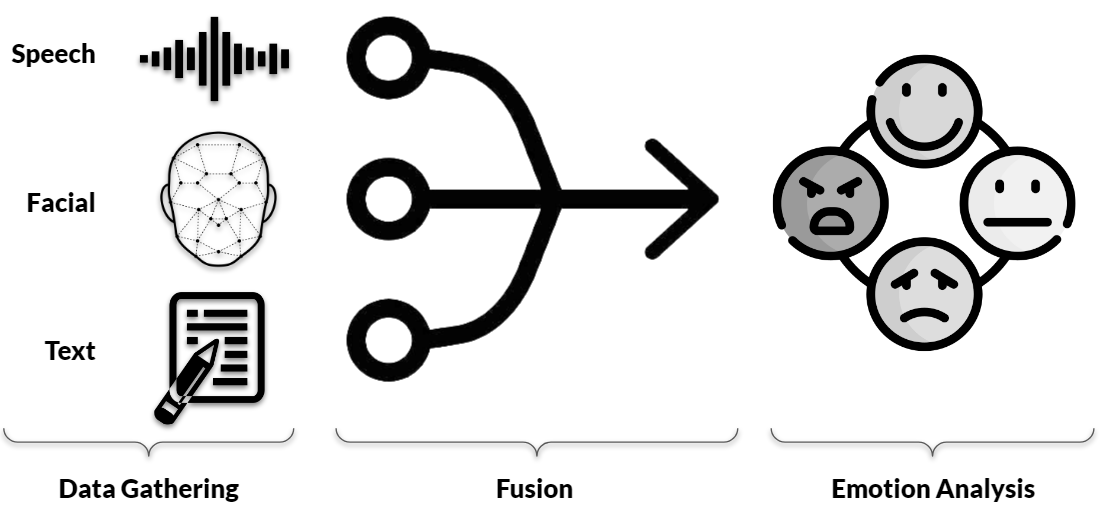
\includegraphics[width=.8\linewidth]{figs/2_state_of_the_art/multimodality.png}
	\caption{Multimodal emotion recognition illustration.}
	\label{fig:multimodal}
\end{figure}

Four main methods of fusion can be used in multimodal systems:
\begin{itemize}
	\item \textbf{Feature level}: This involves combining the features of different modalities and creating a new, high-dimensional feature set.
	
	\item \textbf{Decision level}: Each feature set from different modalities is given as input to different classifiers, and then the prediction results are combined.
	
	\item \textbf{Model level}: The goal of this method is to build a model that captures the complex relationships among the different modalities.
	
	\item \textbf{Hybrid}: This approach combines and takes advantage of the different fusion methods.
	
\end{itemize}

One of the strategies is to use speech transcriptions to understand the context of the utterances correctly and predict their intent. Human oral communication consists of both linguistic and acoustic content, any subtle change in these cues can alter the significance of an expression. However, this approach alone tends to fail, word meanings are very ambiguous, and it fails to capture some low-level features of the speech itself, therefore not achieving the best results. Thus, emotion and sentiment recognition could benefit from considering both linguistic and acoustic features. \citeauthor{BHASKAR2015635} evidenced this improvement by using a hybrid approach based on text and speech mining \cite{BHASKAR2015635}. Similarly, \citeauthor{ser_strategies} also corroborated this idea by using a model that fuses \ac{mfccs} indicators with text transcriptions to predict emotions \cite{ser_strategies}.

In a paper published in \citeyear{Lu2020} by \citeauthor{Lu2020}, it was used a pre-trained end-to-end automatic speech recognition model to extract text features from audio data and combined them with other acoustic features. These features were then fed into a \ac{rnn} with multi-head self-attention, which improved the accuracy of sentiment analysis using only audio data from 67.4\% to 71.7\% on the \ac{iemo} dataset.

In a study by \citeauthor{Handa2021} (\citeyear{Handa2021}), a model was proposed for fusing facial and speech features using a \ac{svm}. The model employed an AlexNet and a deep \ac{lstm} network to extract the facial and speech features, respectively, which were then combined and fed into the \ac{svm} for classification. The model achieved \ac{sota} results on the eNTERFACE’05 dataset for classifying seven emotions, with an overall accuracy of 76.61\% \cite{Handa2021}.

\citeauthor{Yan2021} in \citeyear{Yan2021}, proposed a multi-tensor fusion network with cross-modal modeling with video, audio, and text cues for emotion recognition \cite{Yan2021}. To perform their classification experiences, and obtained results that outperformed their current \ac{sota}, achieving an F1 score of 81.0\% and 81.3\% on the CMU-MOSI and the CMU-MOSEI datasets, respectively.

\section{Emotion Recognition Services}

The widespread use of video conferencing applications has increased significantly during the COVID-19 pandemic, as many people have been forced to communicate remotely. These systems typically use audio and video inputs, as well as text input, to facilitate communication. This growth of video conference usage increased the demand for tools that can improve the virtual communication experience.

In the customer service industry, video conferencing has become very popular, but it can be a challenging task, such as dealing with agitated customers. By providing real-time feedback on the emotions of participants, emotion recognition technologies can prevent problematic situations and evaluate the effectiveness and engagement of the customer service experience.

\citeauthor{Buitelaar2018} in \citeyear{Buitelaar2018} summarized some other known emotion recognition services, that are helping to advance the field, along with their characteristics, displayed below in the table \ref{table:emoServices}. It is visible that most of the services at the time of this study are paid and not open-source \cite{Buitelaar2018}.

\begin{table}[h]
	\centering
	\caption{Emotion recognition services for facial, textural, and speech contents \cite{Buitelaar2018}.}
	\label{table:emoServices}
	\resizebox{.85\textwidth}{!}{%
		\begin{tabular}{@{}lccc@{}}
			\toprule
			Service & Modality & Open-Source & Free\\
			\midrule
			
			\begin{tabular}{@{}l@{}}IBM Watson Alchemy Language \cite{ibmwatson}\\Bitext \cite{bitext2022}\end{tabular} & Text & No & No \\
			
			\begin{tabular}{@{}l@{}}Synesketch \cite{Krcadinac2016}\end{tabular} & Text & Yes & Yes \\
			
			\begin{tabular}{@{}l@{}}Microsoft Cognitive Services \cite{microsoftservice}\\IMOTIONS \cite{kristensen2022}\end{tabular} & Facial & No & No \\
			
			\begin{tabular}{@{}l@{}}Affectiva Emotion API \cite{affectiva}\end{tabular} & Facial & No & Free/Enterprise Editions \\
			
			\begin{tabular}{@{}l@{}}EmoVu \cite{emovuservice}\end{tabular} & Facial & No & No \\
			
			\begin{tabular}{@{}l@{}}Nviso \cite{humanbeaviourservice}\\SkyBiometry \cite{skybiometry2022}\end{tabular} & Facial & No & Limited/Non-Free Editions \\
			
			\begin{tabular}{@{}l@{}}audEERING SensAI \cite{audeering2022}\end{tabular} & Speech & Yes & Free Research Edition \\
			
			\begin{tabular}{@{}l@{}}Good Vibrations \cite{goodvibrations}\end{tabular} & Speech & No & No \\
			
			\begin{tabular}{@{}l@{}}Vokaturi \cite{Vokaturi}\end{tabular} & Speech & No & Limited/Enterprise Editions \\
			
			\bottomrule
		\end{tabular}%
	}
\end{table}


More recently, companies have been working on developing technology for recognizing human emotions, and they are, gradually, adding multimodality to perform emotion analysis. Affectiva \cite{affectiva}, has added the audio modality to their emotion recognition system that initially was only with facial cues. The company primarily uses its technology for market research, but it has also been applied in the automotive industry to monitor drivers' emotions and cognitive states. Microsoft \cite{microsoftservice} has also integrated into their emotion API other modalities over time, such as text and speech. EmoVoice \cite{Wagner13}, is another framework that uses acoustic features of speech to recognize human behavior in real-time, without the need for speech transcription.


\section{Software Tools}

For working and manipulating speech data and also machine learning techniques, different software tools are necessary. Generally, \textbf{Python} \cite{van1995python}, is the most widely used programming language in all machine learning-related tasks, along with \textbf{Pip} \cite{pypi} to install external resources, labeled as Python libraries. Important Python libraries in this area are \textbf{Numpy} \cite{2020NumPyArray} and \textbf{Pandas} \cite{mckinney2010data}, which provide high-level mathematical functions for dealing with big vectors and matrices, \textbf{Matplotlib} \cite{hunter2007matplotlib} and \textbf{Seaborn} \cite{michael_waskom_2017_883859}, for statistical data visualization, \textbf{Keras} \cite{gulli2017deep} and \textbf{scikit-learn} \cite{pedregosa2011scikit}, for implementing and manipulating machine learning algorithms.

For extracting and processing speech, there are several tools available in Python, such as:
\begin{itemize}
	\item \textbf{Librosa} \cite{Librosa}: provides tools for music and audio analysis. It helps to visualize audio signals and extract features using signal processing techniques;
	\item \textbf{OpenSmile} \cite{Eyben2010}: open-source toolkit for audio analysis, processing, and classification that focuses on speech and music applications;
	\item \textbf{COVAREP} \cite{Degottex2014}: an open-source repository of advanced speech processing algorithms that are useful for tasks such as speech analysis, synthesis, and conversion;
	\item \textbf{Spafe} \cite{spafe}: simplifies the process of extracting features from mono audio files and includes various filter bank modules and other spectral statistics;
	\item \textbf{Pydiogment} \cite{ayoubmalek2020}: makes it easy to augment audio files by generating multiple versions with different speeds, tones, and other modifications;
	\item \textbf{Noise Reduce} \cite{tim_sainburg_2019_3243139,sainburg2020finding}: helps to remove noise from time-based signals such as speech.
\end{itemize}

Frequently, \ac{vad*} algorithms are employed in speech processing systems. These algorithms are designed to be highly accurate and efficient in detecting when a user is speaking and filtering out background noise and other non-speech signals. Examples of \ac{vad*} toolkits are:

\begin{itemize}
	\item \textbf{Silero} \cite{SileroVAD}: intended to be used in real-time speech processing applications, it is optimized for performance on a wide range of devices, including mobile phones and other embedded systems;
	
	\item \textbf{Py-webrtcvad} \cite{WebRTCVad}: python interface to the Google's WebRTC \ac{vad*} project, which is an open-source project that provides web browsers and mobile applications with real-time communication capabilities.
\end{itemize}


\section{Summary}

Through the \ac{sota} research, it is possible to state the significant progress over time of not only \ac{ser}, but emotion recognition systems in general. Here are a few key takeaways that emerged from it:

\begin{itemize}
	\item Due to the subjectivity of emotions, the lack of consensus on how to label them, and the need for a large and diverse emotional corpus (e.g. different contexts, genders, languages, etc.), makes the whole process of creating and evaluating an emotion recognition system a very challenging task.
	
	\item Audio feature engineering is a critical aspect of \ac{ser} due to the large variety of features available and the need to carefully select them, including prosodic, spectral, and voice quality features.
	
	\item Traditional feature-based approaches use more classical models and focus mainly on feature selection methods.
	
	\item \ac{dl} strategies with automatic feature extraction capabilities have, in general, outperformed the traditional acoustic feature extraction approach. The most popular models for this are \ac{cnn}, \ac{rnn} (\ac{lstm}), and hybrid \ac{cnn}-\ac{rnn} architectures, with Mel spectrogram as input for them.
	
	\item The field of affective computing, which originally focused mainly on using facial cues to recognize emotions, has seen success in using multiple channels of information (multimodality). This shift has allowed for more accurate emotion recognition, and many current solutions in the market are taking advantage of this approach.
	
	\item There are still areas in which emotion recognition systems need to be improved, such as being able to handle a wider range of input signals and increase reliability. For example, most systems overlook the case of input channels with noise, where the system should weigh each differently, and also, research for online classification contexts is still underdeveloped.
	
\end{itemize}

Overall, there is a significant amount of ongoing research and development that is taking place on emotion recognition systems and has successfully advanced further their capability and reliability, however, there remain a lot of limitations to overcome and areas to improve.
